\documentclass[conference]{IEEEtran}

\IEEEoverridecommandlockouts
% The preceding line is only needed to identify funding in the first footnote. If that is unneeded, please comment it out.

\usepackage{cite, url}
% Enable the following line if you want highlighted hyperlink to citation and references
%\usepackage{hyperref}
\usepackage{amsmath,amssymb,amsfonts}
\usepackage{algorithmic}
\usepackage{graphicx}
\graphicspath{ {./figures/} }
\usepackage{textcomp}
\usepackage{xcolor}

\usepackage{cases}
\usepackage{amsthm}
\usepackage[utf8]{inputenc}
\usepackage[english]{babel}
\newtheorem{theorem}{Theorem}[section]
\newtheorem{corollary}{Corollary}[theorem]
\newtheorem{lemma}[theorem]{Lemma}

% for sequence diagrams and trees
\usepackage{tikz}
\usepackage{pgf-umlsd}
\usepgflibrary{arrows} % for pgf-umlsd
\usepackage{verbatim}
\usepackage{float}
\usepackage[export]{adjustbox}
\usepackage{multicol, blindtext}
\usetikzlibrary{trees}

\usepackage{chngcntr}
\counterwithin{figure}{section}

% for grammar specification
\usepackage[perp]{backnaur}

% for listing grammar example
\usepackage{listings}
\usepackage{alltt}
\usepackage{fancyvrb}
\usepackage{array}
\usepackage{colortbl}
\usepackage{ctable}
\usepackage{booktabs}
\usepackage{multirow}
\usepackage{setspace}

\lstdefinelanguage{permgram} {
                morekeywords={single, array},
                morekeywords={[2]this, root},
                morekeywords={[3]accessor, none, substr},
                sensitive=true,
                morecomment=[l]{//}
}

\lstset{language=permgram,
                basicstyle={\scriptsize\singlespacing},
                keywordstyle={\footnotesize\itshape\color[rgb]{0.1,0.1,0.5}},
                keywordstyle=[2]{\footnotesize\itshape\color[rgb]{0.5,0.1,0.1}},
                keywordstyle=[3]{\footnotesize\itshape},
                tabsize=2,
                basewidth=0.48em,
                commentstyle=\color[rgb]{0.1,0.4,0.1},
                xleftmargin=0.0cm,
                captionpos=b
}

\def\BibTeX{{\rm B\kern-.05em{\sc i\kern-.025em b}\kern-.08em
    T\kern-.1667em\lower.7ex\hbox{E}\kern-.125emX}}
\begin{document}

\title{Integrity Management and Access Control of External Storages using Blockchain Technology 
	\thanks{This research is funded by KONA Software Lab, Ltd.}
}

\author{
	\IEEEauthorblockN{Hasan Mohammad Shahriar}
	\IEEEauthorblockA{\textit{Research and Development} \\
	\textit{Kona Software Lab}\\
		Dhaka, Bangladesh \\
		h.m.shahriar@konasl.com}
	\and
	\IEEEauthorblockN{Saikat Biswas}
	\IEEEauthorblockA{\textit{Research and Development} \\
	\textit{Kona Software Lab}\\
		Dhaka, Bangladesh \\
		saikat.biswas@konasl.com}
	\and
	\IEEEauthorblockN{Muhammad Nur Yanhaona}
	\IEEEauthorblockA{\textit{Research and Development} \\
	\textit{Kona Software Lab}\\
		Dhaka, Bangladesh \\
		nur.yanhaona@konasl.com}
}
\maketitle

\begin{abstract}
The inherent limitation of blockchain technology for storing bulky and confidential information such as files and images is a major obstacle for the technology's adoption as a platform for real-world applications that would otherwise be greatly benefited from the technology's other offerings. As an alternative, this paper presents a novel solution for reliable and secure integration of external document storage systems such as storage clouds and data centers with a blockchain network. In this approach, each document in the external storage is tagged with some blockchain smart contract. The responsibility of document access control, access fee processing, integrity insurance, and user authentication remains in the hands of the blockchain network and external storage systems focus only on storing and delivering documents efficiently. The solution's reliance on the blockchain technology for various control operations related to document access means greater trust and security for these operations. At the same time, it simplifies external document storage systems' design.    
\end{abstract}

\begin{IEEEkeywords}
peer-to-peer computing, distributed information systems, document handling  
\end{IEEEkeywords}

\section{Introduction}
\label{s-intro}
Since its inception in 2008 \cite{bitcoin}, the blockchain technology has gained widespread attention as a transformative technology that can revolutionize many industries \cite{deloitte}. Blockchain based digital currencies such as Bitcoin \cite{bitcoin}, Ether \cite{Wood2014EthereumAS}, and Ripple XRP \cite{David2014TheRP} are already being considered viable alternatives to existing currencies in trade and commerce for their security and ease of transfer. Blockchain smart contracts \cite{FM548} \cite{Wood2014EthereumAS}, on the other hand, have spawned innovative applications in many business and financial sectors due to their capacity of encoding the rules of interaction and ensuring their enforcement.

Central to the appeal of blockchain technology is its maintenance of a distributed ledger of transactions --  called the blockchain -- in a peer-to-peer network of autonomous and anonymous entities. In a blockchain network, all entities are even and none of them is trusted; still, the security and integrity of the transaction ledger can be guaranteed. This feat is achieved by a complete replication of information in all network participants where each participant validates and executes all transactions. As long as the majority of the network participants are honest, the outcome of the transactions, i.e., the state of the blockchain ledger can be trusted \cite{10.1007/978-3-319-56614-6_22}.

The blockchain technology's decentralization of trust through information and processing replication in a, theoretically, infinitely scalable peer-to-peer network is leading innovations and renovations in many application domains where trust and information security are key concerns. However, problem in one area in particular appears to be a major obstacle for blockchain based application adoption. This is the problem of document storage. 

The blockchain technology is inherently unsuitable for storing bulky information such as files and media contents due to the networking and storage cost associated with their management. Peculiarities of blockchain ledger maintenance such as \textit{blockchain reorg} \cite{reorg} further complicates the situation by making direct integration of existing trusted storage solutions with a blockchain network difficult. Finally, public blockchain technologies find the continual preservation and integrity insurance requirement for trustworthy document storage in conflict with their blockchain transaction ledger maintenance incentive where participants are only being paid for extending the ledger of transactions\footnote{by mining transactions into new blocks} and they can join or leave the network at any time.      

Nevertheless, there are some blockchain based or blockchain inspired storage technologies such as Ethereum Swarm \cite{swarm}, Filecoin \cite{filecoin}, Storj \cite{Wilkinson14storja}, and IPFS \cite{ipfs} already available for users. These solutions break down a user's file into a series or hierarchy of data chunks then distribute the chunks to the peer-to-peer network. On a broad level, some of these storage solutions are like traditional distributed hash tables \cite{Maymounkov:2002:KPI:646334.687801} \cite{10.1007/978-3-540-45172-3_4}. Some others are like peer-to-peer file sharing services such as the popular Bittorrent \cite{Pouwelse:2005:BPF:2138958.2138984}. These solutions apply some Bitcoin-like incentive mechanisms on top of these base technologies to motivate the network participants to retain and serve data chunks upon users' request.  

The motivation for these solutions is that they protect the users from vendor locked-in and they offer an overall larger storage capacity compared to existing storage alternatives. However, blockchain based solutions have the common problem that the owner (or user) has to take the responsibility of ensuring persistence and integrity of his/her data in the blockchain by retaining document metadata and issuing periodic audits. Furthermore, despite the combined storage capacity being huge, the download bandwidth can be significantly low as the network peers may be running simple commodity hardware behind low-speed network connections. In addition, designing incentive mechanisms for long-term persistent of documents in a mining based blockchain network is difficult 

Legacy databases of existing applications are also an obstacle for the applications' migration to the blockchain domain. Data stored in proprietary data centers are often confidential that a typical administrator may not be comfortable to put in the hands of anonymous blockchain participants. Further, when existing cloud storage providers \cite{Murty:2008:PAW:1407893} \cite{googleCloud} have already solved the storage capacity, scalability, and cost-effectiveness problems for the clients; there is little motivation for moving data into a blockchain storage.     

We believe, to steer blockchain application innovations, blockchain technology should be supportive of existing storage solutions instead of being their competitors. In other words, the goal should be integrating existing storage technologies with blockchain -- not toppling them. A collaboration of technologies can bring the best of the both worlds. The blockchain technology can ensure integrity of external documents and control access to them according to the transparent governance of blockchain smart contracts and leave the actual storage, delivery, and capacity scaling to a matured storage technology. Here the blockchain technology is ideally suited for its part because information corruption in a blockchain network is very difficult and access rules written in the smart contracts are self-enforcing if integrated properly.

In our scheme, location, signature, access control configuration, upload/download fees and so on metadata information about a document is stored in some blockchain smart contract. We call this contract the {\it document bearer contract}. A user gets access to the externally stored document by interacting with a \textit{Storage Integration Blockchain Gateway} from a blockchain client application. Any conversation with the gateway involves a series of transactions in the blockchain network for updating the document bearer contract and happens following the instructions of some secure interaction protocol. Finally, if the gateway approves the access request then it generates an access token to the external storage that the user uses to upload/download a document with the external storage directly. In case of a download, in particular, the client application verifies document authenticity by locally computing the document signature and matching it against the signature stored in the blockchain before delivering the document to the user. 

Figure~\ref{fig-1} depicts a high-level description of the system architecture of our solution.   
\begin{figure}[h]
\centering
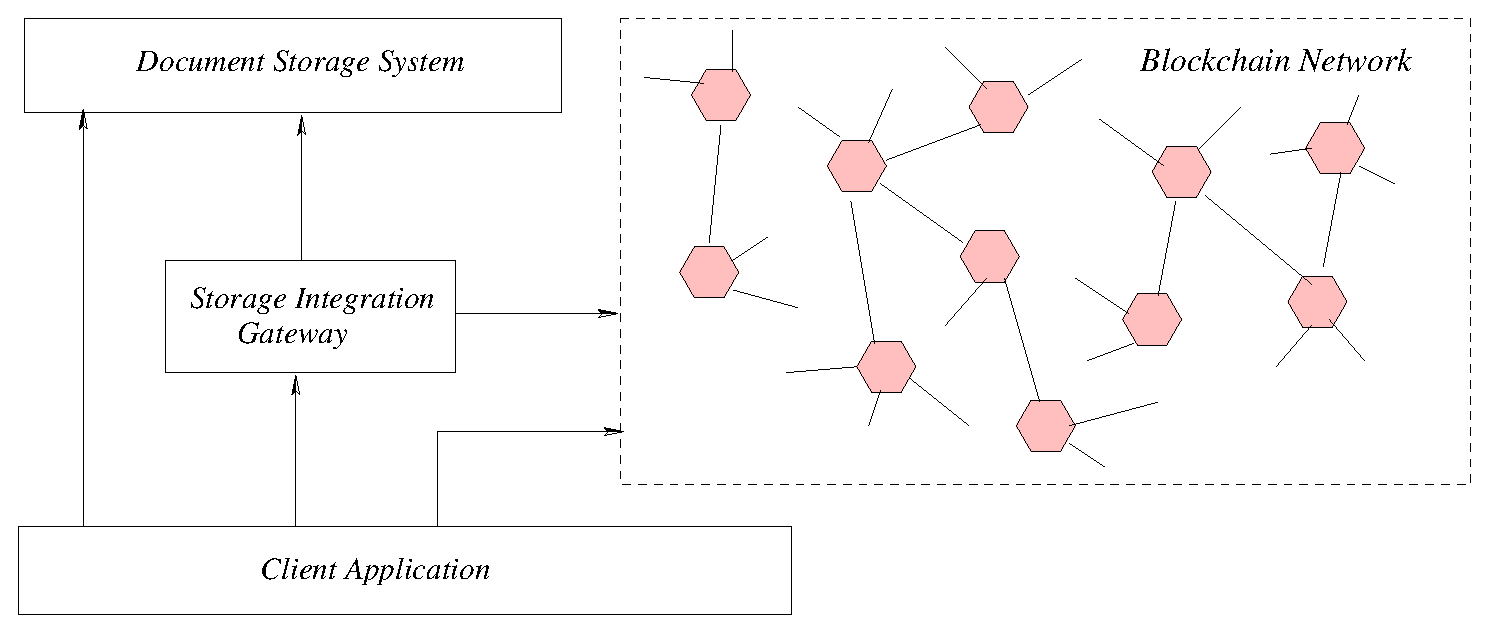
\includegraphics[width=0.48\textwidth]{system-architecture}                    
\caption{External Storage System Integration Model}\label{fig-1}
\end{figure}
Observant readers will notice that the \textit{Blockchain Network} and the back-end \textit{Document Storage} of Figure \ref{fig-1} can scale up to meet users' high-availability and other quality of service needs. However, the same cannot be said about the \textit{Gateway}. If proper care is not taken, its failure can make documents unavailable for client access. We avoided this potential problem by ensuring that the gateway database only contains information derived from the blockchain network. Hence, the gateway can be limitlessly replicated and the same back-end document storage may be interfaced by many gateways at the same time. Furthermore, we support different gateways to be configured differently to charge users for upload and/or download differently based on their quality of service (QoS) and application requirements.

The underlying core innovations that make our solution work are as follows:
\begin{enumerate}
\item Efficient, secure, and accountable document upload-download protocols that support configurable blockchain based payments.
\item A generic document access control configuration paradigm using blockchain smart contracts. 
\item Enforcement of access control rules in storage integration gateways.
\item Fault-tolerant design of the storage integration gateway against blockchain transaction reversal and back-end storage system failures.   
\end{enumerate}         
This paper describes these core innovations and discusses some associated concerns. The rest of the paper is organized as follows:

\subsection{Paper Organization}
Section \ref{s-scope} elaborates on the scope of the external storage integration problem in our modeling, Section \ref{s-updown} describes document upload/download protocols and analyzes their characteristics, Section \ref{s-accr} presents our innovation on blockchain smart contract based document access control policy configuration and its enforcement, Section \ref{s-gate} examines some gateway design concerns, Section \ref{s-rw} discusses some related work on blockchain based/inspired document storage, Finally, Section \ref{s-con} concludes the paper.


\section{The Scope of the Storage Integration Problem}
\label{s-scope}
To discuss the scope of the external storage integration problem, readers first need to understand our vision of responsibility breakdown for blockchain powered applications requiring document storage. For this latter discussion we refer to the model of Figure \ref{fig-1}.

We envision that the application logic of a blockchain powered application (subsequently referred as a \textit{Blockchain Application}) will be stored in the blockchain network in the form of blockchain smart contracts. Information update, payment processing, and any auditing initiated by users' access to the blockchain application will be governed by those smart contracts and reflected as transactions in the blockchain ledger. If we categorize aspects of users' interaction with a blockchain application into \textit{4--As}: \textit{Authentication} of user, \textit{Authorization} of request, \textit{Access} to information, and \textit{Audit} of change; all \textit{4-As} are handled by the blockchain network -- except for the case of access/updating documents such as files and images.

Such documents will reside on one or more external document storage systems. At present, there is no convincing solution for reliable interaction of a blockchain network with an external information system in the literature. Hence \textit{4-As} related to document access/update cannot be handled by the blockchain network as being done for other user interactions. A feasible alternative is that a user's blockchain identity and information in the blockchain ledger set the rules for the user's access to the external storage systems. Then a gateway service interacting with both the blockchain network and the storage systems enforces the \textit{4-As} on behalf of the blockchain network.

To elaborate, a user will identify him/herself with the gateway with his/her blockchain identity and request upload/download of a document in an external storage as additional information associated with some blockchain smart contract. The gateway will check if the blockchain ledger contains permission information that support authorization of the user's request. Then the user and the gateway undergo an access authorization protocol that results in several blockchain transactions for auditing and payment processing. If authorization is successful, the gateway creates a restricted session with the external storage that the user uses to upload/download documents to/from the external storage.

The aforementioned breakdown of responsibilities for external storage access limits the scope of the storage integration problem to two primary activities: 

\begin{enumerate}
\item development of a storage access permission control mechanism that exclusively uses blockchain information, and
\item designing secure, reliable, and accountable protocols for paid or free document upload/download with external storages. 
\end{enumerate}          

Note that although we accept the blockchain network as the veritable source of information for both activities, the storage integration gateway needs to consider that any transaction in the blockchain can be reversed due to blockchain ledger reorganization \cite{reorg}. Consequently, all access control decisions must be made based on the latest state of the blockchain ledger and the upload/download protocols should support rollback and resume. Doing this elegantly is a major design concern for the gateway.

Involvement of the blockchain network in document upload and download with external storages provides a natural mechanism for document integrity checking. During a document upload, a short and unique document signature can be generated from the document content\footnote{for example, a hash of the document byte stream can be the document signature} and stored in the associated blockchain smart contract. During a download, the client application can recompute the signature from the downloaded content and match that with the signature found in the blockchain smart contract. If the two signatures do not match then the document has been modified or corrupted outside the guidance of the blockchain network and the client rejects the document. This simple scheme of using blockchain ledger's immutability to ensure document integrity has been used by others also \cite{stampIO}.  

Subsequent sections chronologically describes the upload and download protocols, the permission control mechanism, and the gateway design.


\section{Document Upload and Download Protocols}
\label{s-updown}
For the discussion of this section, we assume that both document upload and download with the external storage involves blockchain payments. Both protocols heavily use symmetric key cryptography in various steps for information and payment security. We refer the reader to \cite{1455525} for an introduction to cryptography and to \cite{Daemen99aesproposal:} for AES symmetric key cryptography in particular.

\subsection{Quality Criteria for Upload/Download Protocol Design}
We decide on a set of behavioral characteristics for the document upload and download protocols. These characteristics are classified into two groups based on the expectation of the storage integration gateway and that of the user from the protocols. 
From the gateway's perspective the following characteristics are important:
\begin{itemize}
\item Accountability: all actions are traceable in the blockchain.
\item Independence from storage system failure: payment is collected only after all interactions with the storage system are done successfully.
\item Guaranteed Payment: the user can neither fool it to do unnecessary work nor withheld the payment after the work is complete.
\item Fault-tolerance: all local state information should be derivable from the blockchain ledger so that the gateway can restart easily after a failure or data corruption.  
\item Security from Malicious Miners: no mining nodes can snatch the payment intended for the gateway. 
\end{itemize}   
From the user's perspective, on the other hand, the following characteristics are desired from the protocols:
\begin{itemize}
\item Security: no one else can interrupt the storage session intended for the user. 
\item Payment Security: the user must be able to get refunds if he/she does not get the proper service. 
\item Confidentiality: the underlying document cannot be retrieved by others (users or miners) using the audit trail of the protocol execution in the blockchain ledger.
\end{itemize} 
Propriety of both groups of behavioral characteristics is self-evident. Hence we do not elaborate on them further. During the protocol description, we discuss how different aspects of the protocols serve to achieve the mentioned characteristics. 

\subsection{Document Upload Protocol Description}
The document upload protocol is composed of three main phases:
\begin{enumerate}
\item Token deposition by the {\it user}.
\item Document upload processing by the {\it gateway}.
\item Then, payment finalization by the {\it user}.
\end{enumerate}
Each phase of the protocol involves multiple interaction steps among various system components. Figure~\ref{fig:up-proto} presents the sequence diagram of the protocol.
\tikzset{every picture/.append style={transform shape,scale=.60}}
\begin{figure}
  \begin{sequencediagram}
    \newthread{usr}{\it User}{}
    \newinst[1.1]{ac}{ \it Gateway}{}
    \newinst[1.1]{bc}{\it Blockchain Network}{}
    \newinst[1.1]{es}{\it Storage System}{}

    \begin{callself}{usr}{\it Generate Document Key $D_k$}{}
    \end{callself}
    \begin{call}{usr}{\hspace{0.5cm} \it Get Initial Token}{ac}{\it M}
        \begin{callself}{ac}{\it Generate token M with generated key $K_1$}{}
        \end{callself}
    \end{call}
    \begin{callself}{usr}{\it Generate $K_2$ and prepare N}{}
    \end{callself}
    \begin{call}{usr}{\hspace{1cm} \it Upload Document Info and Lock Fee}{bc}{}
    \end{call}
    \begin{call}{usr}{\hspace{0.8cm} \it Upload Document}{ac}{}
        \begin{call}{ac}{\hspace{2.5cm} \it Verify doc size, fee and token M}{bc}{}
        \end{call}
        \begin{call}{ac}{\it Upload document}{es}{\it location Information}
        \end{call}
        \begin{call}{ac}{\hspace{2.5cm} \it Store encrypted location information}{bc}{}
        \end{call}
    \end{call}
    \begin{call}{usr}{\hspace{1.5cm} \it Check upload Status}{bc}{}
    \end{call}
    \begin{call}{usr}{\it Unlock payment with $K_2$}{bc}{}
        \begin{call}{bc}{\it Decrypt $N$ with $K_2$, match with M}{bc}{}
        \end{call}
    \end{call}

    \begin{call}{usr}{\hspace{0.5cm} \it Finalize upload}{ac}{}
        \begin{call}{ac}{\hspace{1.5cm} \it Check payment status}{bc}{}
        \end{call}
        \begin{call}{ac}{\hspace{1.5cm} \it Withdraw fee with $K_1$}{bc}{}
        \begin{callself}{bc}{\it Decrypt $M$ with $K_1$, match caller}{}
        \end{callself}
        \end{call}
    \end{call}
  \end{sequencediagram}
\caption{Sequence diagram of the document upload protocol}\label{fig:up-proto}
\end{figure}
We now describe these steps as parts of the three protocol phases.

\subsubsection{Token Deposition}
The {\it user} generates a document key $D_k$ by performing a hash operation on some document information (document name $D_n$, document uploader blockchain address $DU_{addr}$ and document bearer contract address $DC_{addr}$) to identify the document.
The {\it user} requests the {\it gateway} to generate a token for uploading a document with document size $D_{s}$, document hash $D_{h}$, signature of document hash $DH_{sig}$, $DU_{addr}$ and $D_{k}$. The {\it gateway} validates the input data from the {\it user}. The {\it gateway} generates an AES symmetric key $K_{1}$ and encrypts its blockchain address $G_{addr}$ with the generated key and produces an payment token $M$.
\begin{equation}
\label{eq-u-1}
M = Enc (G_{addr}, K_1)
\end{equation}
The {\it gateway} calculates the document upload fee according to the payment strategy and returns the generated token $M$ and calculated upload fee to the {\it user}.

The {\it user} generates another secret key $K_2$, encrypts the payment token $M$ with $K_2$ to produce an upload token $N$.
\begin{equation}
\label{eq-u-2}
N = Enc (M, K_2)
\end{equation}
The {\it user} performs a transaction to the blockchain with token $M$ and $N$ and other document meta-data. During this operation, the calculated upload fee is also deposited to the blockchain smart contract from the user account.
 
\subsubsection{Document Upload Processing}
After the earlier transaction is mined, the \textit{user} sends the document upload request to the {\it gateway} with the actual document and its meta-data. The {\it gateway} verifies the input data and retrieves the payment token $M$ from the blockchain and verifies that it contains the {\it gateway's} address $G_{addr}$ by performing a decryption on token $M$ with key $K_1$. If all verifications succeed, the {\it gateway} uploads the document to the storage system\footnote{If the storage system allows gateway defined transferable upload sessions for users then the user can do the document upload instead of the gateway.} and stores an encrypted version of the location information in the blockchain. The {\it user} can verify that the document  upload is successful by checking the blockchain.

\subsubsection{Payment Finalization}
After a satisfactory verification of the outcome of upload, the {\it user} issues an unlock payment transaction with the \textit{user's} secret key $K_2$ to the blockchain. The smart contract unlocks the payment if the decryption result of $N$ with provided $K_2$ matches with stored payment token $M$.
\begin{equation}
\label{eq-u-3}
M = Dec (N, K_2)
\end{equation}
The user requests the {\it gateway} to finalize the upload. The {\it gateway} verifies the payment unlock status from the blockchain and issues a transaction to collect the upload payment with its secret key $K_1$. The smart contract decrypts payment token $M$ with $K_1$ and matches the result with the caller address $C_{addr}$. If the address matches with decrypted result, smart contract enables the payment to the caller address.
\begin{equation}
\label{eq-u-4}
C_{addr} = Dec (M, K_1)
\end{equation}

\subsubsection*{Protocol Analysis}
Since it is cryptographically hard to produce an alternative address and key pair that satisfies Equation \ref{eq-u-4}, only the {\it gateway} can collect the payment. On the other hand, since payment is locked until someone supplies proper $K_2$ in the transaction evaluating Equation \ref{eq-u-3}, which is only known to the {\it user}, the {\it user} ensures that the gateway cannot collect the payment until the {\it user} verifies that the document is successfully uploaded. In addition, since the document's location information in the external storage is recorded by the {\it gateway} in the blockchain in an encrypted form, none but the {\it gateway} can interpret this information for future reference. This simultaneously ensures information security and gateway fault-tolerance. Finally, that \textit{user} can issue the required transactions into the designated smart contracts indirectly ensures user authentication.

Note that we did not address the possibility that the upload protocol terminates halfway in the execution for some machine or network failure. This issue can be tackled easily by associating an expiry time with the payment locking transaction. If the protocol fails before the {\it gateway} uploads the document in the external storage system, the user can withdraw the payment after the expiry time. If the failure happens after the document upload in the external storage, then the {\it gateway} can never collect the payment as the user is no longer there to unlock the payment for it. Hence, the {\it gateway} simply removes the document from the external storage in such cases.      

\subsection{Document Download Protocol Description}
The document download protocol being illustrated in Figure~\ref{fig:down-proto} consists of four phases.
\tikzset{every picture/.append style={transform shape,scale=1}}
\begin{figure}
  \label{seq:downloadProtocol}
   \begin{sequencediagram}
    \newthread{usr}{\it User}{}
    \newinst[1.2]{ac}{\it Gateway}{}
    \newinst[1.2]{bc}{\it Blockchain Network}{}
    \newinst[1.2]{es}{\it Storage System}{}

    \begin{call}{usr}{\hspace{0.5cm} \it Get payment token}{ac}{\it  $T_p$, fee amount}
        \begin{callself}{ac}{\it Prepare $T_p$ with generated key $K_{a}$}{}
        \end{callself}
    \end{call}
    
    \begin{callself}{usr}{\it Generate $K_c$, $K_u$ and prepare $T_u$}{}
    \end{callself}
    \begin{call}{usr}{\it Deposit and lock fee}{bc}{}
    \end{call}
    
    \begin{call}{usr}{\hspace{0.5cm} \it Prepare session}{ac}{\hspace{0.1cm} \it $ENC_s$}
        \begin{call}{ac}{\hspace{1.5cm}\it Verify sign and payment}{bc}{\it $T_p$}
        \end{call}
        \begin{callself}{ac}{\it Verify $T_p$}{}
        \end{callself}
        \begin{call}{ac}{\it Generate session}{es}{$S$}
        \end{call}
        \begin{callself}{ac}{\it Generate $K_s$ and prepare $ENC_s$} {}
        \end{callself}
        \begin{callself}{ac}{\it Prepare Hash $H_s$ of $ENC_s$}{}
        \end{callself}
        \begin{call}{ac}{\hspace{0.3cm}\it $H_s$}{bc}{}
        \end{call}
    \end{call}

    \begin{call}{usr}{\hspace{1.0cm} \it verify $H_s$ is the hash of $ENC_s$}{bc}{}
    \end{call}
    \begin{call}{usr}{\hspace{1.0cm} \it Unlock payment with $K_u$, $D_k$, $U_{addr}$}{bc}{}
    \end{call}
    
    \begin{call}{usr}{\it Get session}{ac}{}
        \begin{call}{ac}{\hspace{3.0cm} \it Verify signature and payment status}{bc}{}
        \end{call}
        \begin{call}{ac}{\hspace{3.2cm} \it Withdraw payment with $K_a$, $ENC_{ks}$}{bc}{}
        \end{call}
    \end{call}

    \begin{call}{usr}{\hspace{0.8cm} \it Get encrypted session encryption key }{bc}{$ENC_{ks}$}
    \end{call}
    \begin{call}{usr}{\it Dec($ENC_s$, Dec($ENC_{ks}$, $K_c$))}{usr}{\it $S$}
    \end{call}
    \begin{call}{usr}{\it Download document}{es}{\it Document}
    \end{call}
  \end{sequencediagram}
\caption{Sequence diagram of the document download protocol}\label{fig:down-proto}
\end{figure}
\begin{enumerate}
\item Token deposition by the {\it user}.
\item Download session creation by the {\it gateway}.
\item Payment approval by the {\it user}.
\item Finally, document download by the {\it user}.
\end{enumerate}
The phases are described in more detail below. 

\subsubsection{Token Deposition}
The {\it user} requests the {\it gateway} to generate a document download payment token with the document key $D_k$, document hash $D_{h}$, {\it user's} blockchain address $U_{addr}$, and signature of document hash $DH_{sig}$. The {\it gateway} verifies the input data, generates a payment secret key $K_a$ and encrypts its blockchain address $G_{addr}$ with the secret key and produces a payment token $T_{p}$. 
\begin{equation}
\label{eq-d-1}
T_p = Enc (G_{addr}, K_a)
\end{equation}
The {\it gateway} also calculates the fee according to the payment strategy to download the document and returns the payment token $T_p$ with the calculated download fee to the {\it user}.
After receiving the payment token, the {\it user} generates two symmetric keys $K_c$ and $K_u$. $K_c$ is the common conversation secret shared only with the {\it gateway}. The {\it user} generates an payment unlock token $T_u$ by encrypting $T_p$ with the key $K_u$.
\begin{equation}
\label{eq-d-2}
T_u = Enc (T_p, K_u)
\end{equation}
The {\it user} then issues a download payment transaction to the blockchain with two tokens $T_p$ and $T_u$, and some document related information that deposits the download fee in the blockchain smart contract.

\subsubsection{Download Session Creation}
After the download payment transaction is mined, the {\it user} issues a prepare download session request to the {\it gateway}. During this request, the {\it user} sends document bearer contract address $DC_{addr}$, signed document key $DK_{sig}$, $U_{addr}$, $D_k$, $D_{h}$, and $K_c$. The {\it gateway} validates the input data, retrieves the payment token $T_p$ from the blockchain and verifies by decrypting it with $K_a$ and matching the result with its own blockchain address $G_{addr}$. 
\begin{equation}
\label{eq-d-3}
G_{addr} = Dec (T_p, K_a)
\end{equation}
After successful address verification, the {\it gateway} retrieves the external storage information for the document and requests the {\it storage system} for a session $S$ to download the document. The {\it gateway} then generates a secret key $K_s$,  encrypts $S$ with $K_s$ and produces an encrypted session $ENC_s$. It also encrypts the document key with the common secret $K_c$ and produces an encrypted document key $ENC_{dk}$. 
\begin{equation}
\label{eq-d-4} 
ENC_s = Enc (S, K_s)
\end{equation}
\begin{equation}
\label{eq-d-5} 
ENC_{dk} = Enc (D_k, K_c)
\end{equation}
The {\it gateway} then prepares a hash, $H_s$, of $ENC_s$ and issues a transaction to the blockchain with $H_s$ and $ENC_{dk}$. The {\it gateway} locally stores all input data and returns $ENC_s$ to the {\it user}.

\subsubsection{Payment Approval}
The {\it user} verifies that the hash of $ENC_s$ is stored in the blockchain by the {\it gateway} then issues a transaction to unlock the payment with $K_u$, $D_k$ and $U_{addr}$. The smart contract unlocks the payment by decrypting the unlock token $T_u$ with the secret key $K_u$ provided by the {\it user} and matching the result with the payment token $T_p$. 
\begin{equation}
\label{eq-d-6} 
T_p = Dec (T_u, K_u)
\end{equation}
The {\it user} then issues a request to the {\it gateway} to get the download session encryption key with $D_k$, $DK_{sig}$ and $U_{addr}$. The {\it gateway} verifies the input data and encrypts the session secret $K_s$ with common conversation secret $K_c$ and produces an encrypted session encryption key $ENC_{ks}$.
\begin{equation}
\label{eq-d-7} 
ENC_{ks} = Enc (K_s, K_c)
\end{equation}
The {\it gateway} issues a blockchain transaction to withdraw the payment with the $K_a$ and $ENC_{ks}$. The blockchain smart contract enables the download payment fee to the caller address if the decrypting result of payment token $T_p$ with $K_a$ matches with the caller address. It also stores $ENC_{ks}$ with the download document information in blockchain.

\subsubsection{Document Download}
The {\it user} then collects the encrypted session encryption key $ENC_{ks}$ from the blockchain. The {\it user} first decrypts the encrypted session encryption key $ENC_{ks}$ with the common secret $K_c$ and retrieves the session secret key $K_s$, then decrypts the encrypted session $ENC_s$ with $K_s$ to retrieve the original session $S$.
\begin{equation}
\label{eq-d-8} 
K_s = Dec (Enc_{ks}, K_c)
\end{equation}
\begin{equation}
\label{eq-d-9} 
S = Dec (Enc_s, K_s)
\end{equation}
Finally, the {\it user} downloads the document directly from the storage system using the session $S$.

\subsubsection*{Protocol Analysis}
Payment security for both the {\it user} and the {\it gateway} is ensured as it was in the upload protocol using a pair of encrypted tokens and proper sequencing of the payment related blockchain transactions. Likewise, all steps of the download protocol are also reflected on the blockchain smart contract. This ensures gateway accountability. Further, the {\it gateway} again collects the payment only after completing its interaction with the {\it storage system} to protect itself from any blame related to latter's failure. Finally, information related to the storage session  is recorded in the blockchain in encrypted form while the key $K_c$ for decrypting it is shared securely between the {\it user} and the {\it gateway}. Hence none but these two entities can use the session to get access to the document.

One aspect of the download protocol requires particular attention. This is related to unlocking of the download fee by the {\it user} before he/she can verify that the storage session related information supplied by the {\it gateway} is accurate. Since the {\it user} can be malicious, payment must be unlocked for the {\it gateway} before the {\it user} can decrypt the external storage session related information. However, this ordering opens the possibility that the {\it user} ends up paying for an invalid storage session or dispute its validity when it is actually valid. Therefore, a mechanism is required for automatically resolve any dispute related to external storage session in the blockchain smart contract. This is facilitated by the series of encryption related to the conversation secret $K_c$ and the storage session $S$.

To submit a claim about an invalid session, the {\it user} sends $K_c$ and $ENC_s$ in the blockchain smart contract. That the user has supplied the valid conversation secret is verified by performing the inverse of Equation \ref{eq-d-5} and matching the answer with the document key $D_k$. Since it is the {\it gateway} who did the original transaction, the {\it user} also establishes that the provided $K_c$ value was known to the {\it gateway}. Now the blockchain smart contract itself can compute Equation \ref{eq-d-8} and \ref{eq-d-9} to retrieve the session $S$. It then computes a hash of $S$ and checks if that matches $H_s$ which being stored in the blockchain by the {\it gateway}. If both hashes matches then the {\it user's} session invalidity claim is serious. Then the {\it gateway} maliciousness and external storage  malfunctioning should be investigated. Otherwise, the {\it user's} claim is ignored.          




\section{Document Access Permission Control}
\label{s-accr}
The upload/download protocols of previous section do not launch until the gateway verifies that the requesting user has the proper permissions for accessing the external storage. There are two facets of the access permission verification problem. First, there must be a generic configuration mechanism for encoding the access control policy for associating and accessing external documents with the blockchain smart contracts of an application. Second, there must be an inviolable mechanism for enforcing the said access control policy in the storage integration gateway. Before we discuss these facets, we share our vision about the organization and relationship of the smart contracts of a blockchain application that set the requirements for document access control policy configuration.

\subsection{Blockchain Application Organization}
In our modeling, the smart contracts of a blockchain application form one or more rooted relationship hierarchies. The contracts deployed in the blockchain all come from a set of predefined contract templates and each deployed contract bears an application identifier and a type identifier that relate it to the owning application and the type template respectively.

For example, consider a blockchain application for crowd-funded real-estate assets development. Investors will receive ownership rights on parts of the asset. The asset developer will receive the profit for asset development. The actual development work will be conducted through a series of activities assigned to sub-contractors. In addition, some regulatory agency will be tagged with each asset development project by the local branch of the ministry of land for overseeing purposes. Finally, an investor can trade his/her share on the asset for profit. A probable contract template relationship hierarchy for this description can be as illustrated in Figure~\ref{fig-2}. It is apparent from the description that the root of the relationship in this case is the {\it Project} contract.
\begin{figure}[h]
\centering
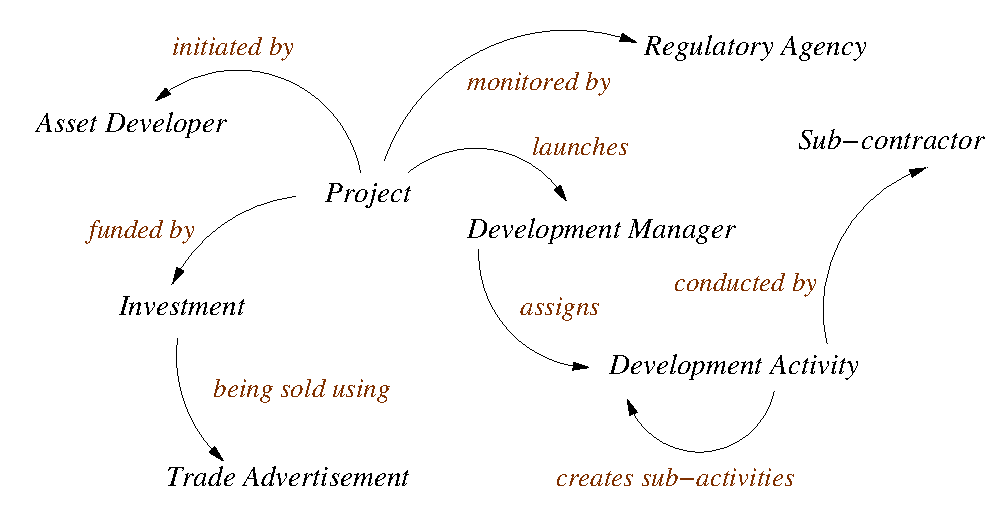
\includegraphics[width=0.48\textwidth]{access-req-example}                    
\caption{An example smart contract relationship hierarchy}\label{fig-2}
\end{figure}

Each contract in the hierarchy may have provision for associating external documents with it. Some of these documents will be public, i.e., accessible to any user upon submission of proper payment. For example, any would-be investor should be able to view documents related to project plan, and the profile of the asset developer and the regulatory agency to make an informed investment decision. Hence these documents should be public. Other documents will be protected and only accessible to users who are somehow related to the smart contracts associated with the documents through the rooted contract relationship hierarchy. For example, once a user invests on a project, he/she will own an investment contract. Only then he/she can access the profile related documents of all sub-contractors who carry the string of of activities for that asset development project and any descriptive documents associated with those activities. However, he/she should not be able to view documents related to the payment negotiated between an assigner of activity and the assignee. Only the involved parties should see these documents. A regulatory agency representative should be able to view all documents associated with the project for proper supervision.    

For associating a document with a smart contract, i.e. document upload, the user must have direct access to the smart contract. For example, only the {\it owner} of an asset developer profile contract should be able to upload profile related documents and link them with his/her contract. He/she should be able to link new documents with a project contract only if he/she is the {\it creator} of the project. Meanwhile, both the {\it assigner} of a development activity and the {\it assignee} can link new documents with the activity. Hence, although in all cases a user must have direct association with the underlying smart contracts, the specific attribute of a contract that relates the user to the contract naturally varies.   

The expectation is that the access control policy configuration mechanism can encode all the various restrictions for document upload and download. Furthermore, the configuration mechanism must be generic as the storage integration gateway is not application specific and may be catering to the needs of multiple blockchain applications simultaneously. In other words, the gateway should not understand attributes such as {\it owner, creator,} and {assigner}; rather, it should interpret a common format of access control policy configuration and apply any configuration blindly.      
 
\subsection{Access Control Policy Configuration}
Our solution for generic specification of access control policies of various blockchain applications is to provide a simple language for expressing how a document bearer contract and the users allowed to access the document are related through the root of a contract relationship hierarchy. There are three components of each permission expression that grants a specific kind of users an specific kind of access to a specific document of a specific type of smart contract:
\begin{enumerate}
\item Source Linkage: a path description that tells how the root of the contract relationship hierarchy can be reached from the document bearer contract.
\item Accessor Linkage: another path description that tells how the root of the contract relationship hierarchy can be reached from the contract holding a reference of the user address.
\item Path Intersection Requirement: a specification that tells to what extent the source and accessor linkages should overlap to grant the user access to the document.     
\end{enumerate}            

\begin{figure*}[t!]
\footnotesize
\begin{bnf*}
\bnfprod{permission} {\bnfpn{docpermissions} \bnfor \bnfes}\\
\bnfprod{docpermissions}{\bnfpn{docpermission} \bnfor \bnfpn{docpermission} \bnfsp \bnfts{;} \bnfsp \bnfpn{docpermissions}}\\
\bnfprod{docpermission}{\bnfpn{doctype} \bnfsp \bnfpn{userpermissions}}\\
\bnfprod{userpermissions}{\bnfpn{userpermission} \bnfor \bnfpn{userpermission} \bnfsp \bnfts{AND} \bnfsp \bnfpn{userpermissions}}\\
\bnfprod{userpermission}{\bnfts{[} \bnfsp \bnfpn{permbits} \bnfsp \bnfts{]} \bnfsp \bnfpn{permexpr}}\\
\bnfprod{permexpr}{\bnfpn{localexpr} \bnfor \bnfpn{remoteexpr}}\\
\bnfprod{doctype}{\bnfpn{attrname} \bnfsp \bnfts{:} \bnfsp \bnfpn{attrmult} \bnfsp \bnfts{--}}\\
\bnfprod{permbits}{\bnfts{r-} \bnfor \bnfts{-w} \bnfor \bnfts{rw}}\\
\bnfprod{localexpr}{\bnfts{(} \bnfsp \bnfpn{attrname} \bnfsp \bnfts{:} \bnfsp \bnfpn{attrmult} \bnfsp \bnfts{)}}\\
\bnfprod{remoteexpr}{\bnfpn{acclink} \bnfsp \bnfts{/} \bnfsp \bnfpn{srclink} \bnfsp \bnfts{/} \bnfsp \bnfpn{overlap}}\\
\bnfprod{acclink}{\bnfts{accessor} \bnfsp \bnfts{(} \bnfpn{attrmult} \bnfsp \bnfts{)} \bnfsp \bnfts{[} \bnfpn{pathdirection} \bnfsp \bnfts{]} \bnfsp \bnfts{=} \bnfpn{path} \bnfsp \bnfts{=} \bnfsp \bnfts{root}}\\
\bnfprod{srclink}{\bnfts{this} \bnfsp \bnfts{=} \bnfsp \bnfpn{path} \bnfsp \bnfts{=} \bnfsp \bnfts{root}}\\
\bnfprod{overlap}{\bnfts{none} \bnfor \bnfts{substr}}\\
\bnfprod{pathdirection}{\bnfts{F} \bnfor \bnfts{R}}\\
\bnfprod{path}{\bnfpn{edge} \bnfor \bnfpn{edge} \bnfsp \bnfts{--} \bnfsp \bnfpn{path}}\\
\bnfprod{edge}{\bnfpn{linkerprop} \bnfsp \bnfts{:} \bnfsp \bnfpn{contracttype} \bnfsp\bnfpn{occurrences}}\\
\bnfprod{attrname}{\bnfpn{string}}\\
\bnfprod{attrmult}{\bnfts{single} \bnfor \bnfts{array}}\\
\bnfprod{linkerprop}{\bnfpn{string}}\\
\bnfprod{contracttype}{\bnfpn{string}}\\
\bnfprod{occurrences}{\bnfes \bnfor \bnfts{[*]}}
\end{bnf*}
\normalsize
\caption{Permission Expression Grammar}
\label{grammar}
\end{figure*}

Figure~\ref{grammar} describes the grammar for permission policy configuration for a document bearer smart contract. The grammar requires that access permissions are specified per document type and individually for each approved user category. For example, assume in the contract relationship hierarchy of Figure~\ref{fig-2}, the {\it investor} of any {\it Investment} contract, the {\it assigner} of an ancestor {\it DevActivity} contract, and any of the {\it representatives} of the {\it RegulatoryAgency} contract can view the {\it license} document of the {\it Subcontractor} contract corresponding to the {\it assignee} of a {\it DevActivity} of the underlying project. Meanwhile, only the {\it owner} of the {Subcontractor} contract can both read and replace (i.e., write) the {\it license} document in the external storage. Then the permission configuration for the {\it license} document should be as described in Listing~\ref{perm-ex}:

\lstset{caption=Example access permission configuration, label=perm-ex}
\lstinputlisting{permission-example.txt}

Our strategy for specifying the access permissions using contract relationship path expressions is a middle ground between access control list (ACL) and role based access control (RBAC) that are typically being used in file systems \cite{Barkley:1997:CSR:266741.266769}. Like RBAC, users gain access to resources because they held specific roles due to their association with specific smart contracts. However, unlike generic roles in RBAC, these roles in our case are indirectly bound to specific resources through some relationship graphs.       

\subsection{Access Control Policy Enforcement}
A storage integration gateway does not need to understand smart contract relationship hierarchies to enforce access control rules specified in the permission expressions of various smart contracts. It only requires that the blockchain network notifies it whenever a smart contract is deployed. In addition, there are APIs to determine the template type of a deployed smart contract, to retrieve the permission expressions governing access to the documents associated with it, and to access metadata related to documents' locations in the external storage. Finally, contracts are required to emit properly formatted events\footnote{An event should contain the addresses of the two contracts whose direct association has been affected by the blockchain transaction, their template type names, and the nature of the update.} in response to blockchain transactions that may affect source or accessor linkages of various documents.\footnote{If we consider a smart contract relationship hierarchy as a directed graph, all relationships may not be traceable from the leaf to the root of the hierarchy. Some relationships may go backward from the root to the leave. Regardless, the events on the audit log should be formatted to support a uniform traversal strategy from the leave to the root.} All these are simple requirements that are easy to satisfy in any typical blockchain network supporting Ethereum Virtual Machine (EVM) specification for smart contracts \cite{Wood2014EthereumAS}.

The gateway monitors these events and derives a document permission database by combining event data and gateway's path expression related query results. This database is like a dynamic ACL database that is automatically being updated in response to new blockchain events. Figure~\ref{fig:perm-ERD} depicts a high level entity relationship diagram of the gateway's document database.
\begin{figure}[h]
\centering
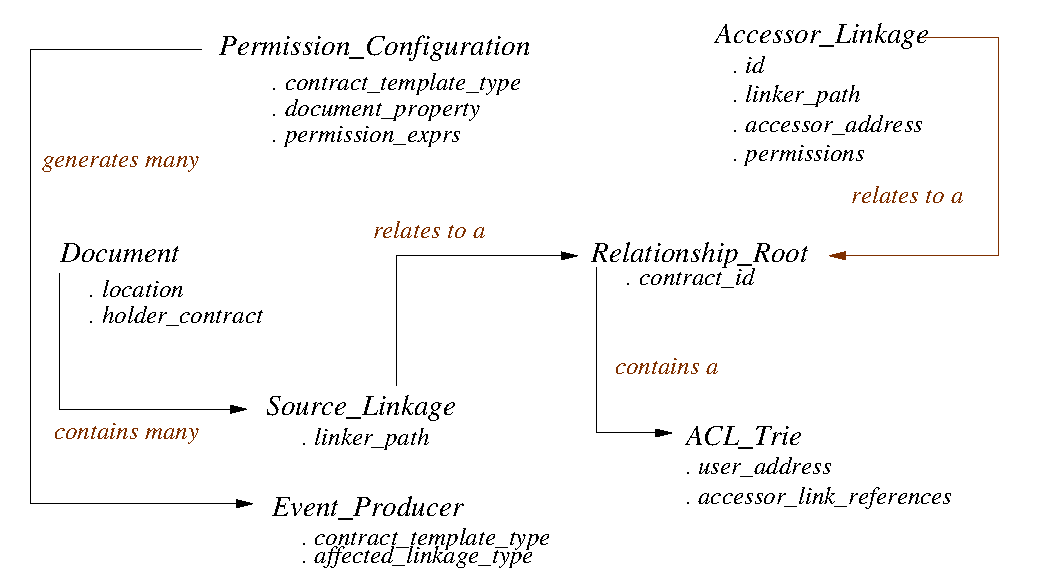
\includegraphics[width=0.48\textwidth]{permission-db}                    
\caption{Entity Relationship Diagram of the Access Permission Database}\label{fig:perm-ERD}
\end{figure}
       
As new smart contracts are being deployed in the blockchain network, the gateway updates contracts' template related information, if not already known, in local database to determine if a contract of this type can affect any document access permission through some source and accessor linkages. In addition, the gateway determines if this type of contract can be a root of any contract relationship hierarchy. For each contract that is a root of a contract relationship hierarchy, the gateway creates an ACL holding Merkle tree (or trie) \cite{6233691} that contains the user addresses that are the endpoints of various accessor linkages originated from the root contract.

If a document is uploaded or an event is published about a change in any property that contributes an edge to the document's paths to various relationship roots, new source linkages are being computed and stored in the database. At the same time, invalidated source linkages are being eliminated. Similarly, if any smart contract property that contributes an edge to users' accessor path to various relationship roots, valid accessor linkages are being recomputed. In addition, the ACL tree entries of the affected users are also being updated.

When a user requests the gateway to undertake an upload/download protocol with the user, the gateway receives the underlying document bearing smart contract's address, the attribute of the smart contract the document refers to, and the user address. Since in case of an upload, the user must be associated with the document bearing smart contract directly, the gateway merely checks the smart contract template description to determine what query to issue in the smart contract to search for the user address. If the requesting user is found registered as a valid uploader then the upload protocol is initiated. Once upload is done, blockchain audit log is traversed to determine new source linkages for that document to existing contract relationship roots. This source linkages are then inserted in the gateway database. If the new document replaces some previously uploaded document then only the location related metadata need to be updated in the gateway database to point to the new document.       

If the user requests for a document download session, the gateway first identifies the ACL trees correspond to smart contract relationship roots reachable by traversing the source linkages of the document. Then it checks if the user's address exists in any of those ACL trees. Then it retrieves all accessor linkages ending at the user address in various ACL trees. Finally, related document source and accessor linkages are compared to decide if they can be combined satisfying any read permission configuration for the document. If any combination attempt succeeds then the user is granted access. If the authorization process fails in any of these steps then the user's request is denied.          
        
Note that although both upload and download protocol initialization request authorization involve local database lookups in the external storage integration gateway, the gateway can be arbitrarily replicated and each replica can resume afresh after a database crash because all information in a gateway database is derived from blockchain ledger data, thus easily recoverable.          
             

             
\section{Storage Integration Gateway Design}
Figure~\ref{fig:gatew} illustrates the internal architecture of the storage integration gateway. The decomposition of the gateway into modules distinguished by their responsibilities comes from good software engineering practices. Their description is outside the scope of this paper. However, we need to understand how the gateway interacts with the blockchain and confidently uses its own database content derived from blockchain ledger information for decision making and internal state assessment given that any information in the blockchain can be reversed due to ledger reorganizations \cite{reorg}. Consequently, the modules connecting the gateway to the blockchain network and the gateway's database design merit some attention.       
\label{s-gate}
\begin{figure}[h]
\centering
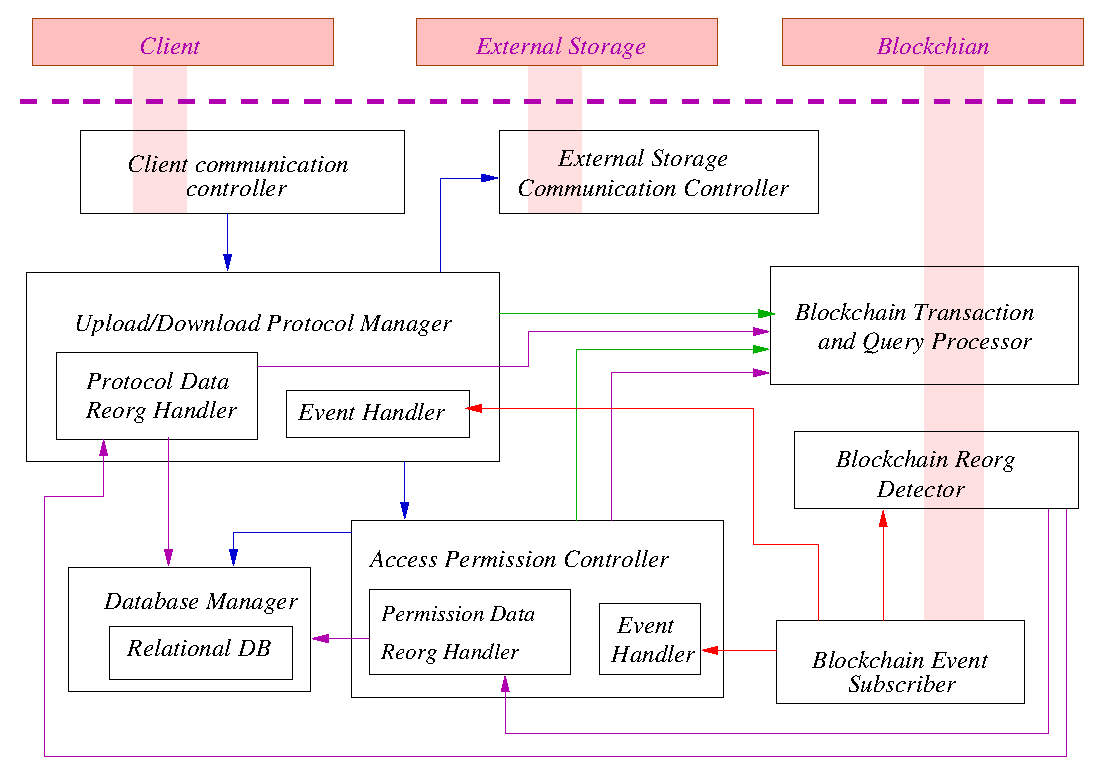
\includegraphics[width=0.48\textwidth]{gateway-design}                    
\caption{Component Breakdown of the Storage Integration Gateway}\label{fig:gatew}
\end{figure}

There are three modules in the gateway for interacting with the blockchain network. {\it Blockchain Transaction and Query Processor} is used during the execution of upload/download protocol for both recording protocol step executions and querying information for protocol initiation and user action validation. Since there may be many gateways in the system that interface the same storage system, protocol transactions issued by a gateway should propagate to others if being mined into blocks. This is achieved by ensuring that any relevant smart contract execution emits events with proper information in the blockchain audit log. The {\it Blockchain Event Subscriber} modules of other gateways capture these events and notify an {\it Event Handler} in their respective {\it Upload/download Protocol Manager} that does database synchronization. Any external action that might change users' access permissions is captured and processed in a similar manner in another blockchain {\it Event Handler} within the {\it Access Permission Controller}.

The gateway issues transactions and receives event notifications by maintaining a connection with some reliable nodes of the blockchain network. At any time, blockchain ledger reorganization can happen in these nodes that may migrate the gateway's transactions to other blocks or throw them away altogether. The gateway must be vigilant and take proper corrective actions in case of such blockchain  reorganizations.

To facilitate proper handling of blockchain reorganization, the gateway retains information about all internal steps of upload and download protocols even after their termination. This information is stored in the gateway database tagged with the hashes (unique block identifiers) of the blocks that recorded the transactions associated with the steps. Similarly, all database entries related to access permission control are also tagged with appropriate block hashes.

If a blockchain reorganization takes place in the nodes the gateway connected with then it becomes aware of the situation through the {\it Blockchain Reorg Detector} module. The module also computes the extent of the reorganization by identifying the blocks that have been dropped in the network. With this information, it initiates two {\it Reorg Handlers} for correcting  upload/download protocol states and for access permission information update. Each {\it Reorg Handler} first retrieves information associated with the blocks from the local database, then searches for their replacement locations in new blocks that caused the chain reorg, and finally determines how to rollback or update the database to bring it to a state consistent with the current version of the blockchain ledger. This database restoration process often involves redoing several transactions in the new blockchain and information update in the external document storage. The underlying algorithm varies with the type of information that is the target of restoration. The process is typically computationally costly and time consuming.                  
       

       
       
\section{Related Work}
\label{s-rw}
To the best of our knowledge, alternative solutions for integrating external storage systems with a blockchain network do not exist. So we describe the well-known blockchain based storage solutions for the sake of completion.   

IPFS \cite{ipfs} is a popular blockchain inspired distributed storage solution. It is basically a distributed hash table (DHT) \cite{Maymounkov:2002:KPI:646334.687801}. The content of each file in IPFS is broken into fixed size blocks and distributed in the network. The hash of a block's content uniquely identify the block in the network. Participant nodes in a IPFS network cache each others data using a Bittorrent \cite{Pouwelse:2005:BPF:2138958.2138984} inspired protocol called BitSwap. In BitSwap, each node has a balance that represents the sum of the ratios of the number of blocks from other nodes it caches compared to the number of its own blocks those other nodes cache. Nodes with large negative balances gradually become isolated in the network by their peers. This encourages a good caching behavior.

Like IPFS, Swarm \cite{swarm} is also a DHT where files are divided into chunks and distributed among the participant nodes in the network. Unlike IPFS, nodes in Swarm receive cryptocurrency payments for serving those chunks to the requester. In addition, a node can make a promise for long term storage of a chunk by issuing a promissory note in the form of a blockchain smart contract. If the node fails to meet its promise, the original owner of the chunk can submit the promissory note as an evidence of misconduct and receive a compensation payment. The integration of payment and penalty in Swarm makes it less likely than in IPFS that nodes will drop chunks.                      

Like Swarm, Storj \cite{Wilkinson14storja} storage network stores files by dividing its content as fixed sized shards and distributing those shards among the network peers. A network peer, called a  farmer, gains Storj coins by serving those shards on user request. Unlike Swarm, there is no built-in provision for contractual agreement between the file owner and the farmer storing a shard. Instead, the owner does periodic audits of the existence of shards using some file metadata. For safety, the metadata for conducting an audit can be stored in some secondary blockchain. Another major difference from Swarm is that all Storj chunks are encrypted by the owner before he/she send them to the farmers.         

Filecoin \cite{filecoin} seamlessly integrates data storage concerns with blockchain network maintenance by making storing of file content a prerequisite for block mining using a scheme called {\it Proof of Retrievability}. Here again a file is divided into fixed sized pieces and distributed among the network peers. In addition, a blockchain ledger is maintained by the peers that records all transactions regarding store and access requests issued by clients. There is a deterministic algorithm for choosing a small subset of existing pieces from different files whose data is used as the input for the next block mining challenge. Therefore, if a peer stores more file pieces, its chance of success in block mining increases. Consequently, peers are inclined to hoard pieces and serving them.   

All these solutions make the file owner responsible for insuring the confidentiality, integrity, and long term availability of his/her file content. In addition, since pieces of a file coming from different parts of the network need to be stitched together before serving, file download latencies can be significant and unpredictable. Finally, since the loss of a single piece corrupts the entire file, all pieces must be stored with the same level of redundancy. That may increase cost of storage significantly.




\section{Conclusion}
\label{s-con}
This paper serves as a comprehensive description of our solution for securely integrating document storage systems such as storage clouds and data centers with a blockchain network such that access to those storage systems is governed by policies regarding payments and access permissions specified in blockchain smart contracts. The solution positions a gateway system in between the storage and the blockchain network that enforces these policies regarding storage access. The gateway is designed to be easily replicable and tolerant to internal failures.

The solution's philosophy is that regarding the management of bulky and, in particular, static information such as documents and images, the blockchain technology should take the responsibility for access control, payment processing, document integrity insurance, and auditing while a storage technology should hold the coveted information and provide access to them. This partitioning of responsibility provides the flexibility of using a mature storage technology in blockchain powered applications. This provides an added security and accountability for document processing that currently only the blockchain technology can offer. Our solution is quite different from the blockchain based storage alternatives that store bulky information directly within the blockchain network using complex mining incentive mechanism and still burdens the user with information availability and integrity insurance.             

There are three aspects of our solution: first, cryptographically secure and accountable protocols for handling information upload and download with the external storage; second, a generic access permission control strategy for launching those protocols; finally, a mechanism to deal with reversal of blockchain transactions related to the protocols and access control. The paper described all three of them. There are significant room for improvement in all three aspects, in particular, for performance betterment. That will be a target of future research.         
 

 
\bibliographystyle{plain}
\bibliography{references.bib}

\end{document}
